%%% -*- coding: utf-8 -*-
\newpage

\chapter{Theory and technical background}
\label{chap:theory}

\section{Convolutional Neural Networks}\label{sec:CNN}
Neural Networks
Image classification: ImageNet\footnote{\url{http://www.image-net.org/}}
Audio classification: Audioset\footnote{\url{https://research.google.com/audioset/}}

vanishing gradient problem. with deep cnns

\section{The VGG Convolutional Neural Network}\label{sec:VGGish}

The VGG Convolutional Neural Network~\cite{simonyan2014VGG} was designed for the ImageNet Challenge in 2014, where it won the first and second place in localization and classification tasks. It's input is a 224$\times$224 RGB image. The main contribution of this network is that is showed that even with a very small receptive field (3$\times$3, which is the smallest size to capture the notion of left/right, up/down and center, by increasing the depth of a network, it could still outperform all other CNN based methods at the time.

This architecture has 6 configurations with different depths that are connected to two Fully Connected (FC) layers, two of 4096 channels and a final one with a 1000 channels (The Image Net challenge had a 1000 classes), followed by a soft-max layer that outputs the predicted class.
The configuration of the fully connected layers is the same in all configurations. All hidden layers used rectification (ReLU)~\cite{krizhevsky2012relu} non-linearity. Figure \ref{fig:vgg16} shows the most popular variation, the VGG-16 (Configuration D) and its layers, as described above.

\begin{figure*}[!ht]
    \centering
    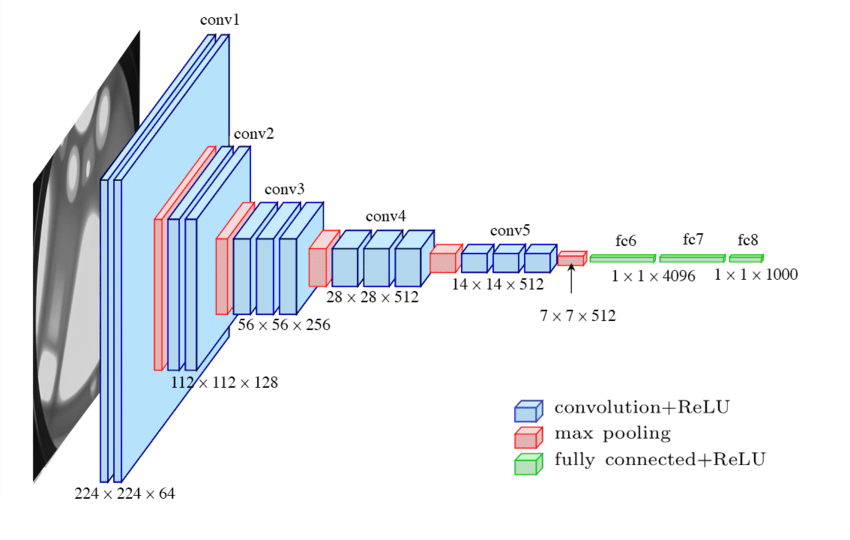
\includegraphics[width=0.95\textwidth]{img/vgg16.png}
    \caption{VGG-16 architecture, image authors are Ferguson et. al.\cite{ferguson2017vggimage}.}
    \label{fig:vgg16}
\end{figure*}

\section{VGGish}\label{sec:VGGish}
VGGish~\cite{simonyan2014VGG}

The VGGish is a variation of the VGG-11 (Configuration A), created by the authors of the YouTube8m dataset ~\cite{abu2016youtube}, with some modifications to perform audio (spectogram) classification and embeddings generation).

Specifically, the input size was modified to 96$\times$64 for log mel spectogram audio inputs. The last group of convolution and maxpool layers were removed. In order to created a compact embedding layer, the 1000 channels wide FC layer at the end was changed to a 128-wide FC layer. This final layer does not have an non-linear activation.

\section{The Inception Convolutional Neural Network}\label{sec:Inception}

The Inception Convolutional Neural Network or GoogLeNet, ~\cite{szegedy2015Inception} was designed for the ImageNet Large-Scale Visual Recognition Challenge in 2014, it features many techniques in order to increase efficiency of deep CNNS.

In order to achieve this increased efficiency, the authors created a module to capture as much information as possible, both in local and global context, by using multiple kernel sizes in the same convolutional layer. To optimize for computational cost and speed, the creators also avoided naively stacking layers, for it is computationally expensive.

The solution proposed by the authors of the inception CNN is to use compute multiple filters in the same level, with varying convolutional filter sizes.

The ``Naive'' inception module, as shown in Figure \ref{fig:naive-inception} consists on a convolutional layer using 3 different filter sizes, 1$\times$1, 3$\times$3 and 5$\times$5. Along with a max pooling operation. The outputs are then concatenated by the end of the inception module.

\begin{figure*}[!ht]
    \centering
    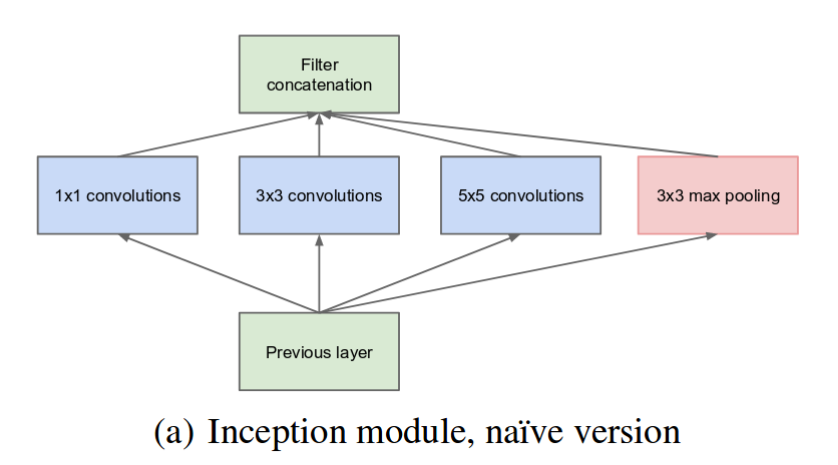
\includegraphics[width=0.95\textwidth]{img/naive-inception.png}
    \caption{The ``Naive'' inception module, image authors are Szegedy et. al.~\cite{szegedy2015Inception}.}
    \label{fig:naive-inception}
\end{figure*}

In order to reduce computational costs further, the authors added 1$\times$1 convolutions after the max pooling step and before the 3$\times$3 and 5$\times$5 convolutions. By doing this the authors reduce the amount of processing done by reducing the quantity of input channels before the convolutions. This improvement was named ``The inception module with dimension reduction'' and it is represented in Figure \ref{fig:}.  

\begin{figure*}[!ht]
    \centering
    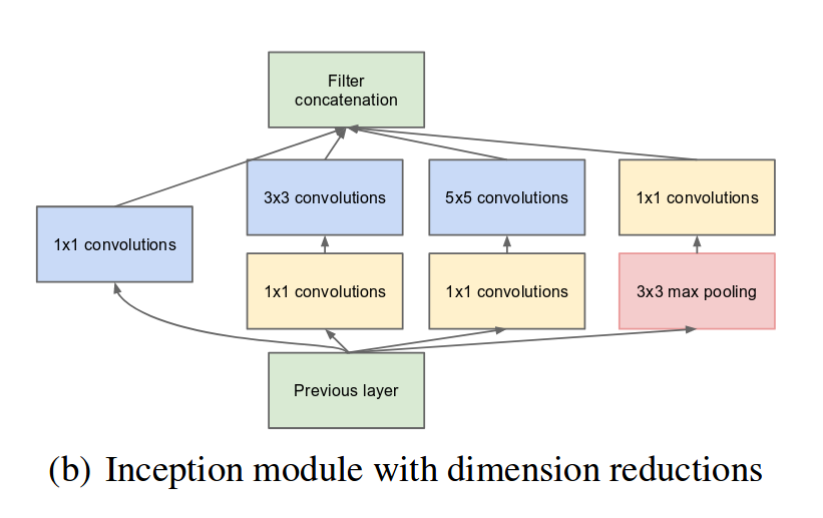
\includegraphics[width=0.95\textwidth]{img/inception-module.png}
    \caption{The inception module with dimensional reduction, image authors are Szegedy et. al.~\cite{szegedy2015Inception}.}
    \label{fig:inception}
\end{figure*}

By stacking 9 inception modules with dimension reduction and using 2 intermediate classifiers, essentially computing prediction values and using these values to compute auxiliary losses, which are then used to compose the final loss in the training process in order to avoid the vanishing gradient problem.

As shown in Figure \ref{fig:inception-architecture} It is still deeper (it has 22 convolutional layers) than the deepest VGG configuration (with 19 convolutional layers).

\begin{figure*}[!ht]
    \centering
    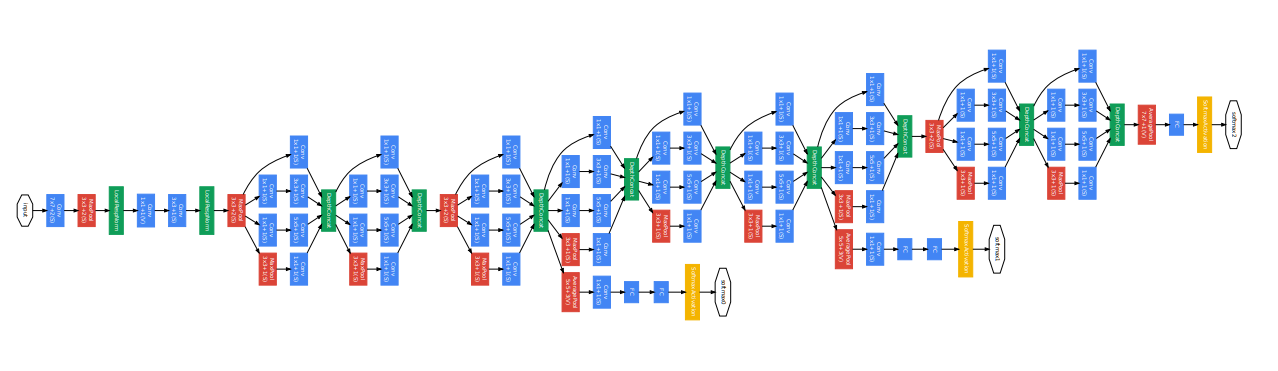
\includegraphics[width=0.95\textwidth]{img/inception-architecture.png}
    \caption{The complete inception convolutional neural network, image authors are Szegedy et. al.~\cite{szegedy2015Inception}.}
    \label{fig:inception-architecture}
\end{figure*}

InceptionV2 and InceptionV3 networks~\cite{szegedy2016rethinking}
For the inceptionV2 computational efficiency was improved by factorizing the convolutions, convolutions with 5$\times$5 size kernels were factorized into two 3$\times$3 sequential convolutions, this improves computability (because 3$\times$3 convolutions use 2.78 times less operations than 5$\times$5) while actually improving performance. They also factorized the 3$\times$3 convolutions into one 1$\times$3 and 1$\times$3 convolutions. These factorized convolutions are performed on the same input to avoid excessive dimension reduction (information loss).

The InceptionV3 CNN used all the upgrades of the InceptionV2, and improved performance further by incorporating the RMSProp Optimizer \cite{tieleman2017rmsprop}, factorized 7$\times$7 convolutions ( 1$\times$7 convolutions followed
by 7$\times$1 convolutions.), batch normalization in the Auxillary Classifiers, and Label Smoothing (It is a modification in the loss function that prevents the network having high confidence in a class) for preventing overfitting.


% RMSProp Optimizer.
% Factorized 7x7 convolutions.
% BatchNorm in the Auxillary Classifiers.
% Label Smoothing (A type of regularizing component added to the loss formula that prevents the network from becoming too confident about a class. Prevents over fitting).

The Inception CNNs continued to improve further with InceptionV4 and Inception-ResNet ~\cite{szegedy2017inceptionv4}, but we will not detail them here for they are not used in the scope of this work.



\section{Feature Fusion}
\label{sec:feature_fusion}

Since we are using information from two different domains, image and audio, it is also important to think how one can fuse information from both these domains without . 
Which method is best to fuse the information from these different domains.

Snoek et al. \cite{snoek2005featurefusion} presents two main strategies for information fusion in semantic video analysis: 
\begin{itemize}
    \item \emph{Early fusion} methods (Figure \ref{fig:early-fusion}), which works directly with the extracted features.
    \item \emph{Late fusion} methods (Figure \ref{fig:late-fusion}), which operates on classification outputs from specialized models.
\end{itemize}

% late fusion comes at cost of training time
In the work by Snoek et. al.\cite{snoek2005featurefusion}, the Late fusion approach tends to give better performance on most semantic concepts (multilabel video classification) at the cost of increased computability costs. However, the authors also conclude that the late and early fusion approaches should be compared are per concept (in a multilabel situation).%, which one can generalize to per task in binary tasks.

\begin{figure*}[!ht]
    \centering
    \begin{subfigure}[b]{0.55\textwidth}
        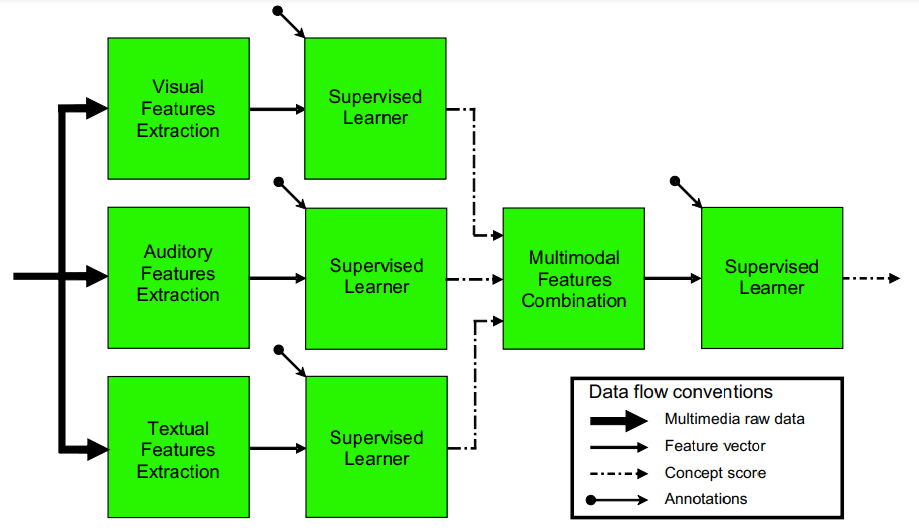
\includegraphics[width=0.94\textwidth]{img/late-fusion.png}
        \caption{The late fusion approach, in it there is a machine learning model for each unimodal feature and a final model to fuse the outputs of each unimodal model.}
        \label{fig:early-fusion}
    \end{subfigure}
    \begin{subfigure}[b]{0.44\textwidth}
        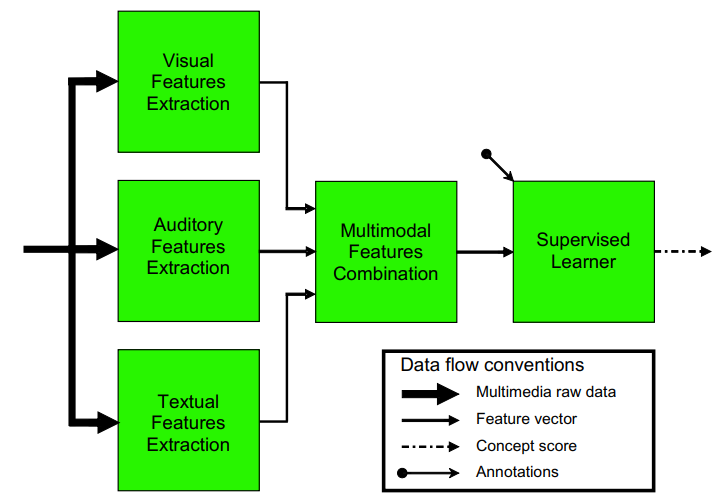
\includegraphics[width=0.94\textwidth]{img/early-fusion.png}
        \caption{The early fusion approach, it uses a single multimodal machine learning model to both aggregate and classify all features.}
        \label{fig:late-fusion}
    \end{subfigure}
    \caption{The late and early fusion methods for feature fusion. Image authors are Snoek et. al.~\cite{snoek2005featurefusion}.}
\end{figure*}
